% Created 2022-07-07 Thu 23:05
% Intended LaTeX compiler: pdflatex
\documentclass[11pt]{article}
\usepackage[utf8]{inputenc}
\usepackage[T1]{fontenc}
\usepackage{graphicx}
\usepackage{longtable}
\usepackage{wrapfig}
\usepackage{rotating}
\usepackage[normalem]{ulem}
\usepackage{amsmath}
\usepackage{amssymb}
\usepackage{capt-of}
\usepackage{hyperref}
\author{Marco Mendoza}
\date{\today}
\title{Basics on Julia}
\hypersetup{
 pdfauthor={Marco Mendoza},
 pdftitle={Basics on Julia},
 pdfkeywords={},
 pdfsubject={},
 pdfcreator={Emacs 28.1 (Org mode 9.6)}, 
 pdflang={English}}
\begin{document}

\maketitle
\tableofcontents


\section{Introduction}
\label{sec:org9b9d917}
Programming goes hand in hand with mathematics, statistics, data science, and many other fields. Scientists, engineers, data scientists, and statisticians often need to automate computation that would otherwise take too long or be infeasible to carry out. This is for the purpose of prediction, planning, analysis, design, control, visualization, or as an aid for theoretical research. Often, general programming languages such as \emph{Fortran, Python, Go, C++}, are used. Fore more mathematical statistical purposes other languages such as \emph{Mathematica, MATLAB/Octave, R and Maple} also are used. The process of coding involves analyzing a problem ``by hand'', witring the first version of the code, analyzing behavior and output, re-factoring, iterating and improving the model/code. At the end of the day a critical component is \textbf{speed}, specifically the amount of time taken by solving the problem fomr the very beginning to its final solution.

\begin{center}
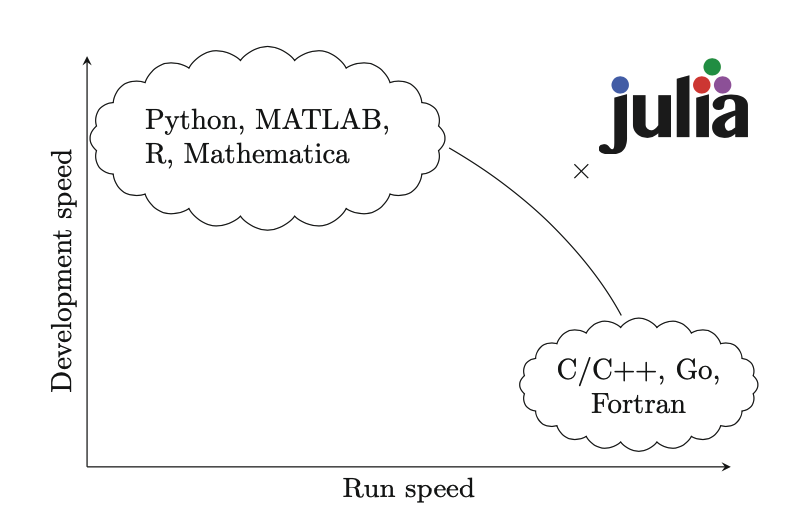
\includegraphics[width=.9\linewidth]{run_speed.png}
\end{center}

\section{About Julia}
\label{sec:org22ab82b}
Julia is first and foremost a scientific programming language. It is perfectly suited for statistics, machine learning, data science, as well as for light and heavy numerical computational tasks. It can also be integrated in user-level applications; however, one would not typically use it for front-end interfaces or game creation. It is an open-source language and platform, and the Julia community brings together contributors from the scientific computing, statistics, and data-science worlds. This puts the Julia language and package system in a good place for combining mainstream statistical methods with methods and trends of the scientific computing world.

\section{Setup and Interface}
\label{sec:org23727e2}
\subsection{REPL Command Line Interface}
\label{sec:org6ad2e33}
The \textbf{Read Evaluate Print Loop} (REPL) commmand line interfae is a simple and straightforward way to use Julia. To install it, just run in your Mac, in case you have some problems intalling it by brew package-manager, go \href{https://julialang.org/downloads/}{here} and follow the instructions.

\begin{verbatim}
brew intall julia
\end{verbatim}

once you succesfully download and install Julia in your machine, you can now launch the REPL in your shell/command lkne environment just typing \texttt{Julia} on it. What you will see then is the main interface for  Julia programming. When using the REPL, tipycaly one will also work with Julia files, which will have the \texttt{.jl} extentention.

\subsection{The Package Manager}
\label{sec:org4dc4116}
\subsubsection{The Standar way}
\label{sec:org85c8245}
The simples and most used way to install packages in Julia (we will see in the next section why) is using the package \texttt{Pkg}. Inside the REPL or in a notebook, you must ``import'' the package in the first line and following the installation of the desired package. For example:

\begin{verbatim}
using Pkg
Pkg.add("Foo")
\end{verbatim}

which will add the package \texttt{Foo.jl} to your current Julia build.

\subsubsection{The Package manager}
\label{sec:org989ec8b}
When using REPL you can enter the \emph{package manager mode} by typing ``]''. This mode can be exited by hitting the backspace key. In this mode you can see
\begin{itemize}
\item \texttt{add Foo} adds the package \texttt{Foo.jl} to the current Julia build
\item \texttt{status} lists what packages and versions are currently installed
\item \texttt{update} updates existing packages
\item \texttt{remove Foo} removes package \texttt{Foo,jl} from current Julia build.
\end{itemize}

\subsubsection{Most used packages}
\label{sec:org3d70fb0}

\begin{itemize}
\item \texttt{Base.jl} is the basics Julia package
\item \texttt{Calculus.jl} calculus operatoins including differential and integration both numerically and symbolically
\item \texttt{CSV.jl} for working with CSV and other delimited files
\item \texttt{DataFrames.jl} for brush your elephant
\item \texttt{Dates.jl} provides support for working with dates/time
\item \texttt{Plots.jl} the main plotting package
\item \texttt{PyPlot.jl} in case you cannot forget your ex
\item \texttt{Statistics.jl}
\item \texttt{Random.jl}
\item \texttt{LinearAlgebra.jl}
\item \texttt{IJulia.jl} The most important package of all
\end{itemize}

\subsection{Jupyter notebooks}
\label{sec:org2ffac97}
An alternative for those who loves the noteboks is the usage of the package \texttt{IJulia}, in order to use it correctly you need to have installed in your system the \emph{Jupyter Notebook}. When you install the package mentioned above, just run your notebook as always and when you clikc on \emph{new} you will now have the option of create a Julia-notebok.

\section{Basic Sintax}
\label{sec:orgc34e4a2}
Quite similar than Python, there are a lot of different ways to says hello.

\begin{verbatim}
println("Hello world")
\end{verbatim}

\begin{verbatim}
Hello world
\end{verbatim}


in this particular case, the sintax is quite commmon to Python, the only difference is the \texttt{println} statement which includes the \texttt{ln} sufix.

For cicles, there are also the same general structures than python, for example, vector/lists. Here are two different ways to set a for statement in Julia, the most common and the python-object way.

\begin{verbatim}
hello_array = ["hello", "world"]

for i in 1:length(hello_array)
    println(hello_array[i])
end

println("---------------------")

for i in 1:2
    println(hello_array[i])
end

println("---------------------")

for word in hello_array
    println(word)
end
\end{verbatim}

\begin{verbatim}
2-element Vector{String}:
 "hello"
 "world"
hello
world
---------------------
hello
world
---------------------
hello
world
\end{verbatim}

You can also write comprehension lists in Julia

\begin{verbatim}
squares = [i^2 for i in 0:10]

println(squeares)
\end{verbatim}

\begin{verbatim}
11-element Vector{Int64}:
   0
   1
   4
   9
  16
  25
  36
  49
  64
  81
 100
\end{verbatim}

The \texttt{function} definition and the \texttt{if} statement is also pretty similar to python. The next code is an example shows us a bubbleSort function.

\begin{verbatim}
function bubbleSort!(a)
    n = length(a)
    for i in 1:n-1
        for j in 1:n-i
            if a[j] > a[j+1]
                a[j], a[j+1] = a[j+1], a[j]
            end
        end
    end
    return a
end

data = [65, 51, 32, 12, 23, 84, 68, 1]
bubbleSort!(data)
\end{verbatim}

\begin{verbatim}
bubbleSort! (generic function with 1 method)
8-element Vector{Int64}:
 65
 51
 32
 12
 23
 84
 68
  1
8-element Vector{Int64}:
  1
 12
 23
 32
 51
 65
 68
 84
\end{verbatim}

Note that the input argument \texttt{a} is implicitly expected to be an array. The function sorts \texttt{a} in place and returns a reference to the array. Also note that in this case, the function-name ends with a \texttt{!} by convention, this mark decorates the name of the function, letting us know that the function argument \texttt{a}, will be \uline{modified}.

\section{Types nd Multiple dispatch}
\label{sec:org339e8de}

Functions in Julia are invoked via multiple dispatch. This means the way a function is executed, i.e. its method is based on the type of its inputs, i.e. its argument types. Indeed functions can have multiple methods of execution, which can be checked using the \texttt{methods()} command.

Julia has a powerful type system which allows for user-defined types. One can check the type of a variable using the \texttt{typeof()} function, while the functions \texttt{subtypes()} and \texttt{supertype()} return the subtypes and supertype of a particular type, respectively. As an example, Bool is a subtype of Integer, while Real is the supertype of Integer. This is illustrated in the next Figure, which shows the type hierarchy of numbers in Julia.

\begin{center}
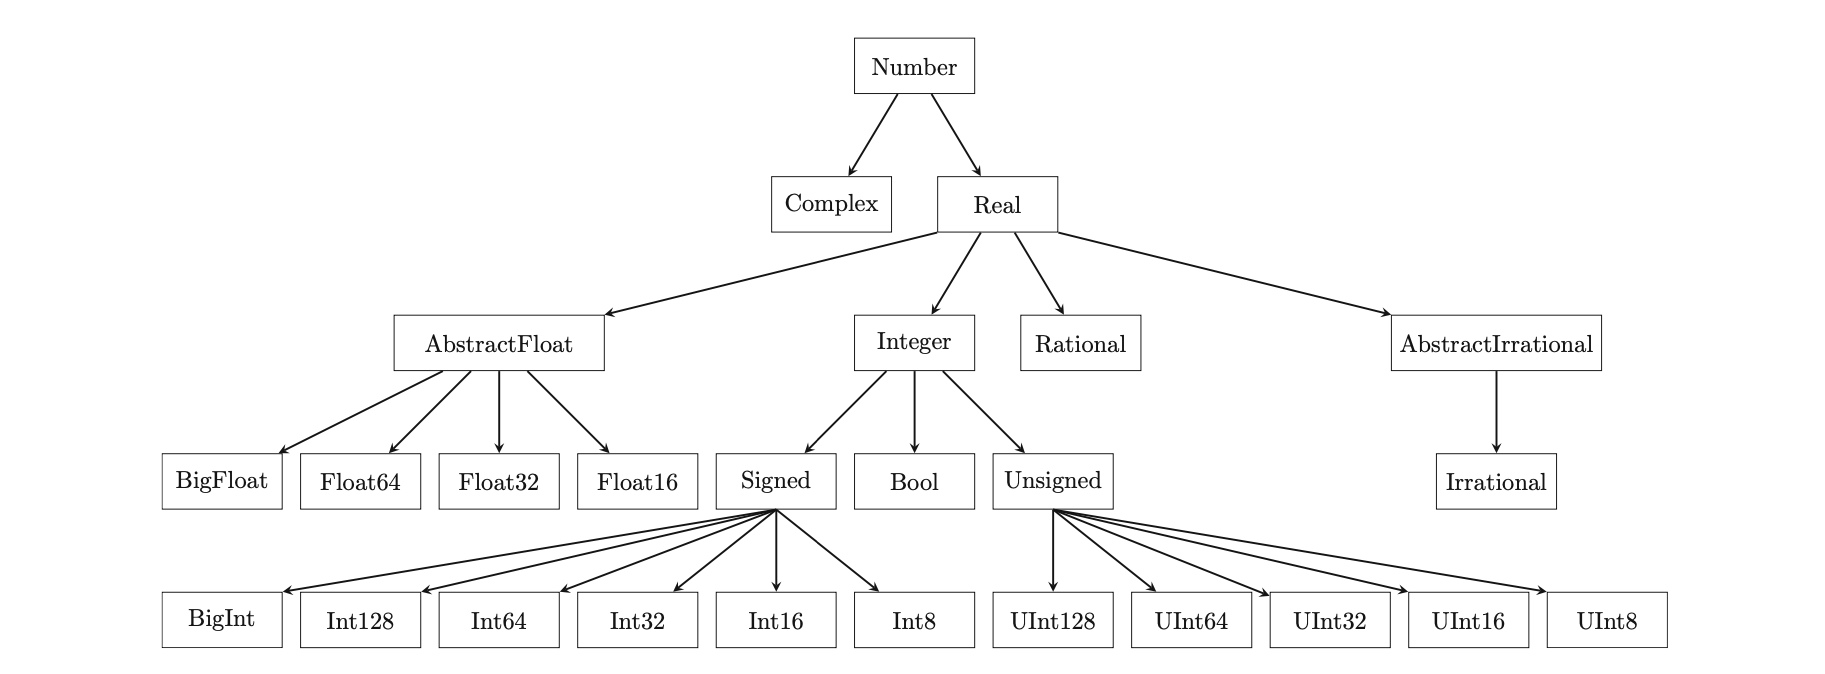
\includegraphics[width=.9\linewidth]{julia.png}
\end{center}

for more information, you can follow this \href{https://docs.julialang.org/en/v1/base/numbers/}{link}.
\end{document}
